%\section{Transition Rate Matrix describing movement of electrons}
%\section{Movement of electrons}
%\section{Electron densities}
\section{Analysis of a Chemical Reaction}

Since each clustered matrix can be written as $S\inv T$, with the familiar meaning of $S$ as overlap matrix and $T$ as coupling matrix, we can deduce that \textbf{each} clustered system possesses some kind of (more or less) rebinding effect (not only restricted to receptor-ligand systems).
The meaning of this effect has to be interpreted for each system individually.
We present a different system (chemical/physical), describing the movement of electron densities of a given molecule.
\\

Formic acid is a molecule consisting of one carbon atom $C$, two oxygen atoms $O$ and two hydrogen atoms $H$.
In hydrocarbons and in the vapor phase, it consists of hydrogen-bonded dimers rather than individual molecules. \marginpar{ref}

In such a system, reactions between the individual molecules can be take place. An $H$ atom which is attached to an $O$ atom/nucleus moves to the $O$ atom of another molecule and vice versa.
These reactions are possible because of the (double) proton tunneling, see Schild\cite[Chapter 4]{schild2013}. \marginpar{ref} %caused/provoked
According to these reactions, changes in the electron density can be observed. %observed/computed
\\

Why is this electron density $\pi(t)$ time-dependent? \marginpar{pericyclic} \marginpar{metastable sets} \marginpar{coherent sets}

\begin{figure}[!ht]
	\centering
	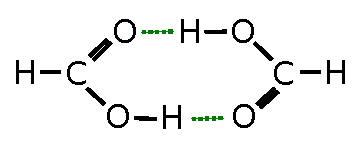
\includegraphics[width=0.4\textwidth]{figures/formic_acid_dimer.eps}
	\caption{Electron densities are measured in a system of formic acid dimers.}
	\label{fig:acid_dimer}
\end{figure}


%measured/computed(?)
Such a system can be described by a Markov chain, where the transition matrix $P$ consists of the (time-dependent) electron densities. %possible b/c electron densities sum up to 1???
Each of the different time-steps yields its own transition matrix. Then $P$ can be constructed of these matrices such that it is reversible.
 
 As $P$ is compound of several transition matrices, it possesses many dominant eigenvalues. However, for each of the individual transition matrices, $4$ metastable regions can be identified. 
%Electron densities of these reactions have been measured/computed(?) and can be described by a Markov chain
Clustering $P$ into $4$ metastable sets using PCCA+ yields the following transition rate matrix: %(though many large eigenvalues?)
%The following transition rate matrix has been obtained from a large reversible process by clustering with PCCA+:
%from experimental data by clustering with PCCA+:
\begin{equation*}
Q_c = 
\begin{pmatrix}
-2.0040  &  1.6859  &  0.1490  &  0.1690 \\
1.6192 &  -2.0010  &  0.1724  &  0.2095  \\
0.1451  &  0.1747 &  -1.9548  &  1.6350  \\
0.1632  &  0.2106  &  1.6217  & -1.9955
\end{pmatrix}.
\end{equation*}
Since it has been clustered with PCCA+, we assume that this system includes/contains \textbf{no} large rebinding effect (objective of PCCA+: make membership functions as crisp as possible).
Applying optimization problem $\eqref{eq:optimization}$ to this matrix, we find out that the minimal rebinding effect included in this system is given by
%\begin{equation*}
%	\det(\Sopt) = 0.9994,
%\end{equation*}
\begin{equation*}
\det(\Sopt) = 1,
\end{equation*}
and thus the optimal overlap matrix is the identity matrix.
\\

Unfortunately, this bound gives us no information about how much rebinding is obtained by the clustering.
This bound can be explained by the reversibility of the clustered system, $\Vert DQ_c - Q_c^T D \Vert_1 = 0$, and theorem \ref{thm:reversible_trivial}.
\\

However, from observing the given membership functions $\chi$ in figure \ref{fig:electron_membership}, we notice that they are not very crisp, but rather overlapping. %can already see
\begin{figure}[!ht]
	\centering
	\includegraphics[width=0.6\textwidth]{figures/electrons/electrons_membership2.eps}
	\caption{Membership functions created by PCCA+}
	\label{fig:electron_membership}
\end{figure}

%However, since we are given the membership functions $\chi$ and the stationary distribution $\pi$ of the original process, 
Knowing the membership functions $\chi$ and the stationary distribution $\pi$ of the original process, we can compute the \textbf{real} rebinding effect by
\begin{equation*}
%S = D\inv \chi^T \diag(\pi, \dots, \pi_{500}) \chi.
\Sreal = D\inv \langle \chi, \chi \rangle_\pi
\end{equation*}
and thereby obtain
\begin{equation*}
\det(\Sreal) = 0.2925.
\end{equation*}

We have already seen before, that the minimal rebinding $\det(\Sopt)$ is not always a good estimation for the real rebinding and in particular is useless if the clustered process is reversible. %especially for systems close to reversible

However, it is astonishing that in this clustered system, there is actually so much real rebinding included. That was unexpected, since clustering with PCCA+ aims for rather crisp membership functions which would result in few rebinding.

Thus, even though the estimation $\det(\Sopt)$ was bad in that example, we can interpret the meaning of the actual rather high rebinding caused by the clustering.

%Ausblick: time-dependent clustering.. i.e. PCCA+ can yield different membership functions, making the Q_c more non-reverible sometimes and then implying a slightly better estimation for rebinding

%This example represents the existence of the rebinding effect in any kind of clustered processes.
%Originally, it was motivated by receptor-ligand systems, but is also occurs in other systems.
%Depending on the system the meaning of ``rebinding'' has to be interpreted corresponding to the context.
In that example, movements of electron densities around a given molecule have been considered.
%Thus, a strong overlap (=strong rebinding) can be explained by ...
The existence of the $4$ metastable conformations located around the $O$-molecules is plausible, since hydrogen is attracted to $O$.
However, these conformations are strongly overlapping. That can be explained by the rebinding effect. A hydrogen atom which is about to leave its $O$-atom and wandering to the next, possesses still a large probability to ``go back''/return to its original connected $O$.

%\begin{figure}[!ht]
%	\centering
	%\includegraphics[width=0.1\textwidth]{figures/formic_acid.eps}
%	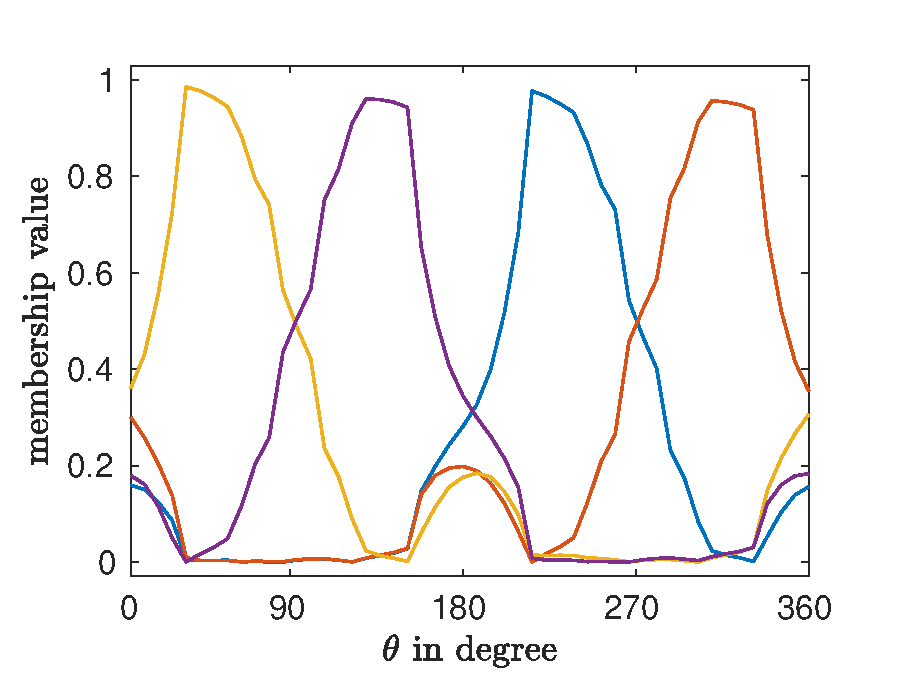
\includegraphics[width=0.6\textwidth]{figures/electrons/electrons_membership.eps}
%	\caption{Membership functions created by PCCA+}
%	\label{fig:electron_membership}
%\end{figure}

%electron density = describes trajectories of electrons (aufenthaltsdauer/ Zerfallsrate)


%This bound, being really high, gives us only few informations about the real rebinding effect; it could be either large or small.
%In this case, we didn't get much information from the optimization problem, even though the examined system is to a rather large extent non-reversible:
%\begin{equation*}
%	D Q_c = 
%	\begin{pmatrix}
%		-2.0249  &  1.6911  &  0.1547  &  0.1792 \\
%		1.6154 &  -1.9846  &  0.1743  &  0.1949  \\
%		0.1500  &  0.1769  & -1.9608  &  1.6339  \\
%		0.1725  &  0.1964  &  1.6225 &  -1.9915
%	\end{pmatrix}
%\end{equation*} vs
%\begin{equation*}
%	Q_c^T D = 
%	\begin{pmatrix}
%	  -0.0250  &  0.0209 &   0.0019 &   0.0022 \\
%	  -0.0316  &  0.0388 &  -0.0034 &  -0.0038 \\
%	  -0.0721  & -0.0850  &  0.9421 &  -0.7850 \\
%	  0.0841  &  0.0958  &  0.7912  & -0.9711
%	\end{pmatrix}
%\end{equation*}
%and the resulting deviation %\marginpar{which norm?}
%\begin{equation*}
%\Vert DQ - Q_c^T D \Vert_1 = 1.7577.
%\end{equation*}
%In order to evaluate the quality of this bound, we compare it to the real rebinding effect $\det(S_{\textrm{real}})$ obtained by the membership functions which has been used to perform this clustering. Since the original process and the membership functions (by PCCA+) are known, it is possible to compute the real rebinding effect.
\newpage

%What is the meaning of this matrix and of the included rebinding effect?